% !TEX encoding = UTF-8 Unicode

\documentclass[a4paper]{article}

\usepackage{color}
\usepackage{url}
\usepackage[T2A]{fontenc} % enable Cyrillic fonts
\usepackage[utf8]{inputenc} % make weird characters work
\usepackage{graphicx}

\usepackage[english,serbian]{babel}
%\usepackage[english,serbianc]{babel} %ukljuciti babel sa ovim opcijama, umesto gornjim, ukoliko se koristi cirilica

\usepackage[unicode]{hyperref}
\hypersetup{colorlinks,citecolor=green,filecolor=green,linkcolor=blue,urlcolor=blue}

\usepackage{algorithm}
%\usepackage{algorithmic}
\usepackage{algpseudocode}


%\newtheorem{primer}{Пример}[section] %ćirilični primer
\newtheorem{primer}{Primer}[section]
\newtheorem{defi}{Definicija}[section]
\newtheorem{teo}{Teorema}[section]



\begin{document}

\begin{titlepage} 
	\centering
	{\scshape\LARGE Matematički fakultet \par}
	\vspace{1cm}
	{\scshape Master rad\par}
	\vspace{0.5cm}
	{\huge\bfseries Detekcija kolizije u realnom vremenu\par}
	\vspace{0.5cm}
    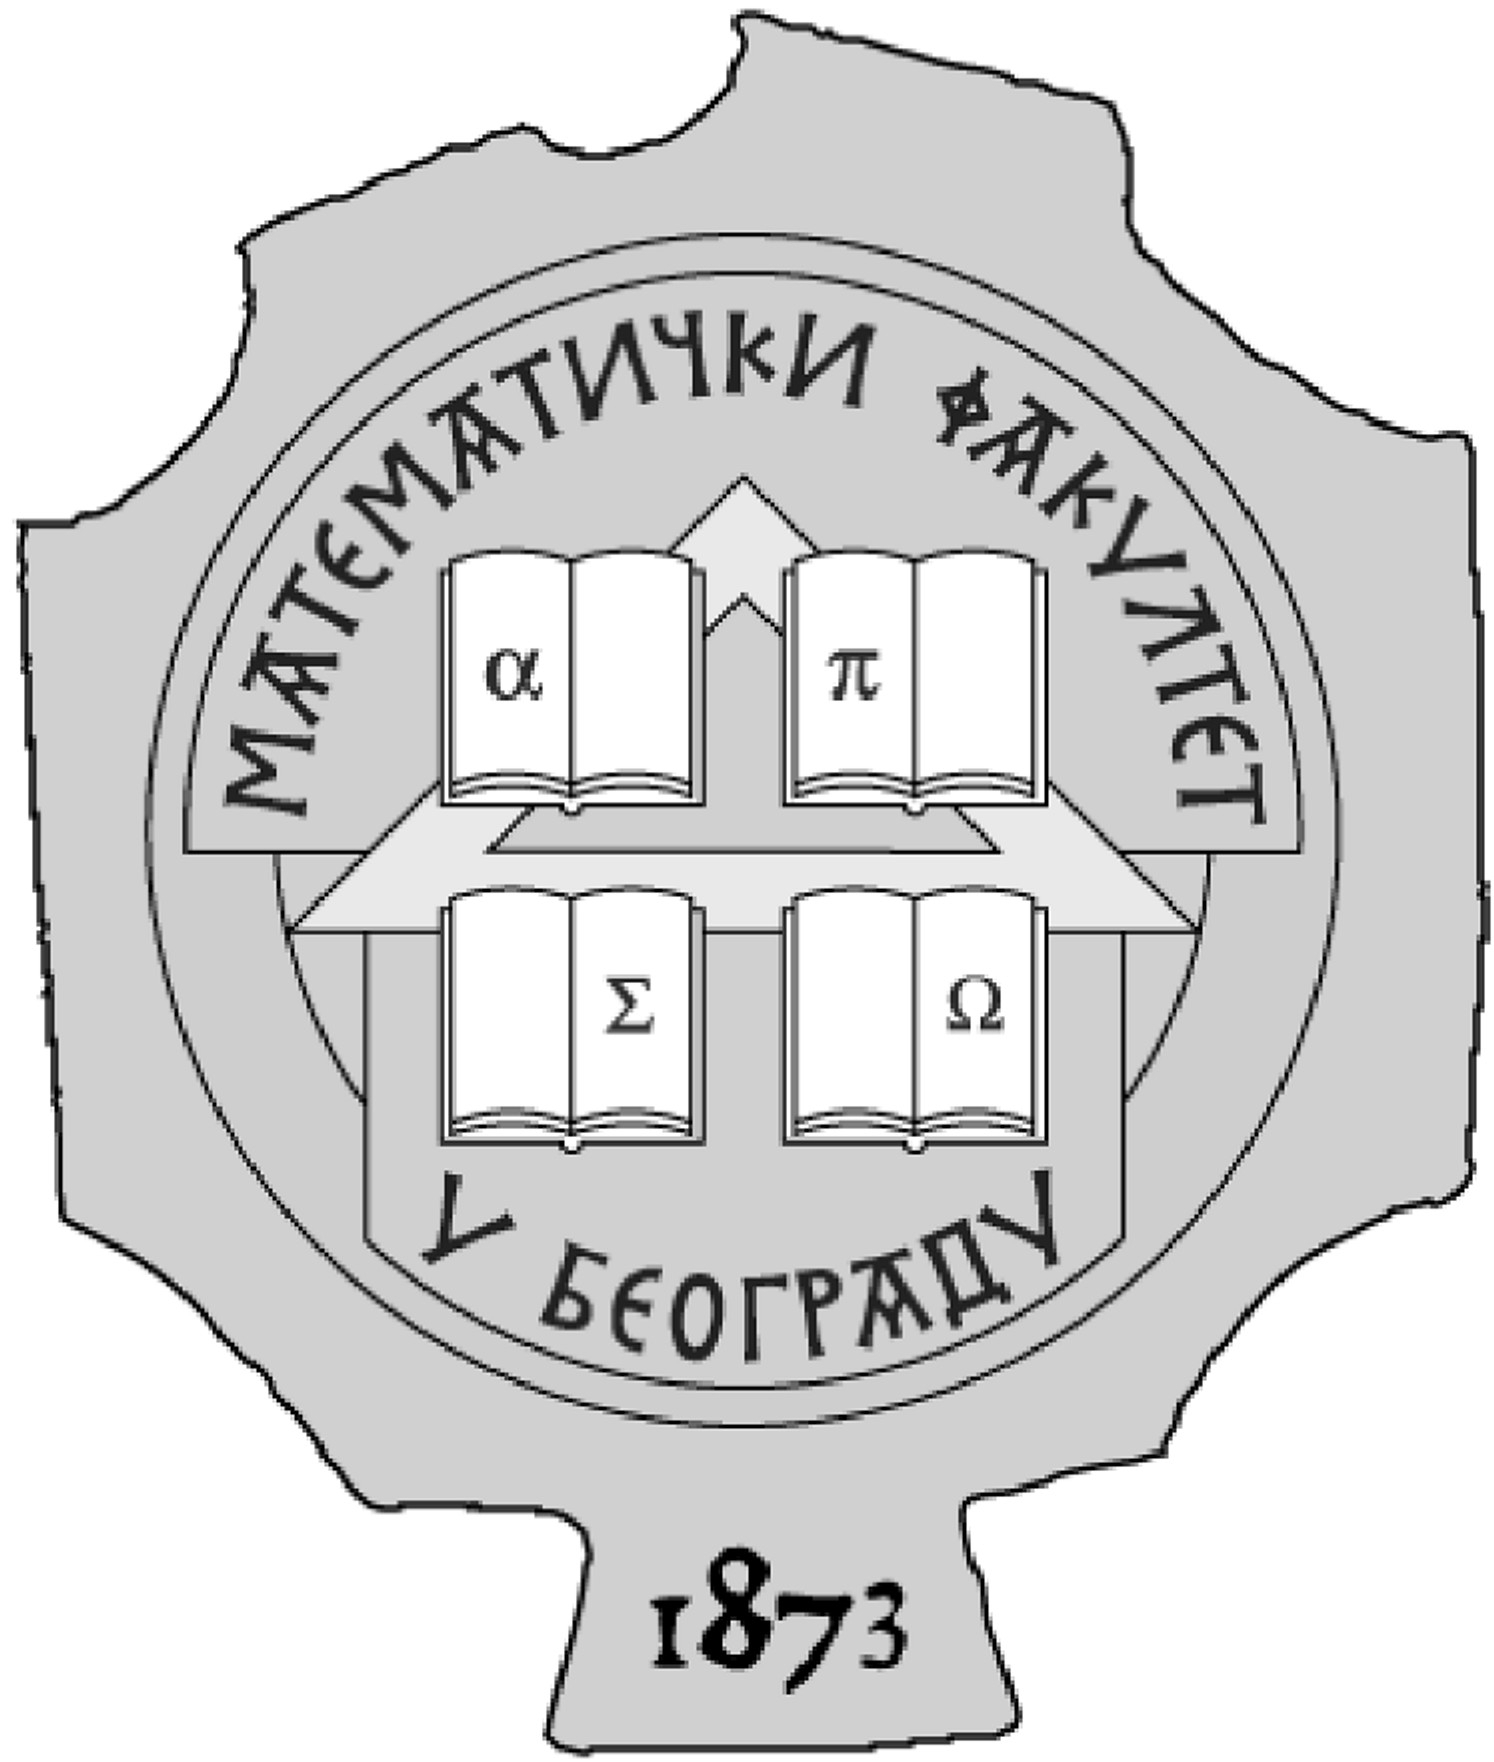
\includegraphics[width=0.45\textwidth]{logo-matf.jpg}\par\vspace{1cm}
    Student:\par
	{ Nikola Dimitrijević\par}
	\vfill
	Mentor:\par
    dr Vesna Marinković
	\vfill
    
    Članovi komisije:\par
    dr Predrag Janicić\par
    dr Ivan Cukić


	\vfill

% Bottom of the page
	{\large \today\par}
\end{titlepage}

\abstract{
Abstrakt.

\tableofcontents

\newpage

\section{Uvod}
\label{sec:uvod}
Uvod.

\section{Motivacija}
\label{sec:naslov1}
Detekcija kolizije je ključan deo svakog pogona igre (eng. {\em game engine}), a danas ga svaka velika
video igra koristi. Industrija video igara svake godine raste \cite{game_industry},
toliko da ima veći prihod od filmske i muzičke industrije zajedno! Zaista, industrija igara ima prihod od
115 milijardi dolara naspram 41 milijardi filmske i 17 milijardi muzičke industrije \cite{music} \cite{movie} \cite{game_industry}.
Posledice neispravnosti igara nisu dramaticne poput neispravnost softvera u avionskoj ili automobilskoj industriji, ali 
se svakako jasno odražavaju negativno na prihod.
Korisnici očekuju visok stepen doteranosti video igara, pa bi postojanje velikog broja bagova 
 obeshrabrilo potencijalne kupce. Na slici \ref{fig:batman} se vidi bag gde je igrač propao kroz 
 mapu, a na slici \ref{fig:horse} igrač ne može da se popne na konja pošto on lebdi u vazduhu.

Pojavljuju se na tržištu VR rukavice koje simuliraju dodir virtuelnih objekata, a za njih je 
detekcija kolizije svakako presudna. Potrebno je bar 1000 puta u sekundi pružiti povratnu informaciju
da bi simulacija dodira bila uverljiva \cite{haptic}. 

\begin{figure}[h!]
\begin{center}
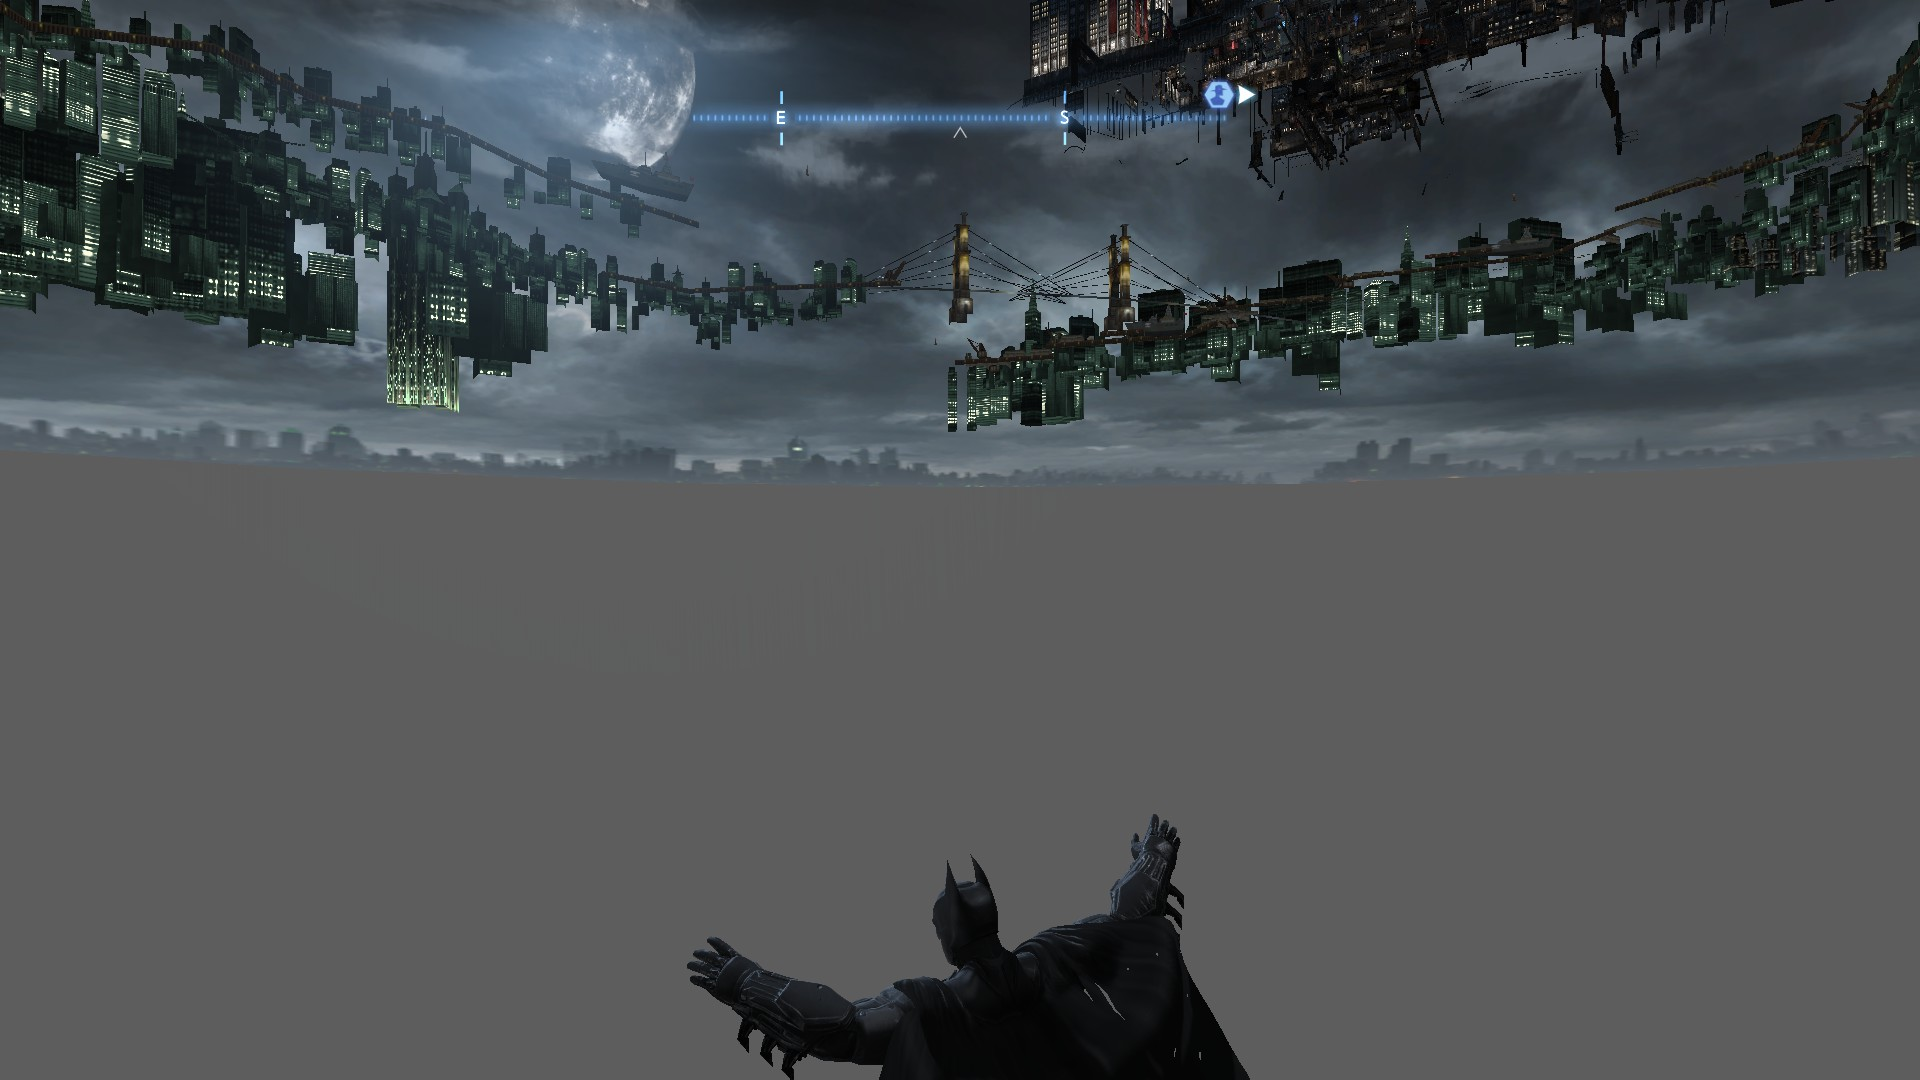
\includegraphics[scale=0.15]{batman.jpg}
\end{center}
\caption{Propadanje kroz mapu.}
\label{fig:batman}
\end{figure}

\begin{figure}[h!]
	\begin{center}
	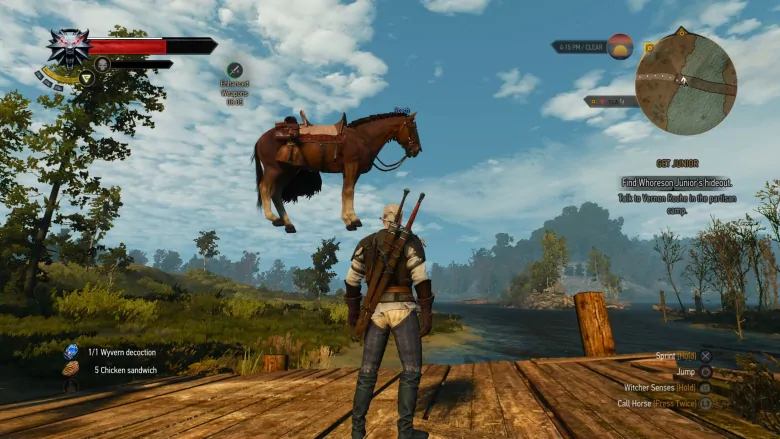
\includegraphics[scale=0.35]{horse.png}
	\end{center}
	\caption{Levitirajući konj.}
	\label{fig:horse}
\end{figure}

Problem detekcije svih parova kolizije je u najgorem slučaju kvadratne složenosti i od toga se ne može pobeći,
ali uglavnom ih ima mnogo manje od gornje granice.
Razlog zahteva da se izvršava u realnom vremenu kod interaktivnih programa je očigledan, ali je takođe
potrebana mogućnost da se što češće i efikasnije utvrde kolizije. Filmovi nisu interaktivan sadržaj i zato
je učestalost osvežavanja slike od 24hz, uz korišćenje zamućivanja pokreta (eng. {\em motion blur}),
dovoljno dobro za većinu ljudi. Standard za igre na konzolama je barem 30hz, a na desktop računarima 
cilj je barem 60hz. Za VR je potrebno barem 90hz inače će lako prouzrokovati dizorijentaciju, mučninu i druge
neželjene efekte \cite{importance}.

Nema najboljeg algoritma detekcije kolizije za svaki mogući slučaj. 
Neki su dobri za uniformno raspoređene objekte u prostoru, ali loši kada su svi na jednom mestu, 
dok su drugi indiferentni što se tiče raspršenosti i više im je bitna brzina kretanja objekata.
Takođe, isti algoritam može imati značajno bolje performanse ako su njegovi parametri dobro 
izabrani za neku hardversku arhitekturu ili scenario. 
Te okolnosti su inspirisale razvoj programa koji omogućava brzo i interaktivno menjanje različitih
algoritama detekcije kolizije, postavljanje njihovih parametara kao i posmatranje performansi.


\section{Glavne karakteristike}
\label{sec:naslov2}

\subsection{Faze}
Broadphase, narrowphase, bounding box.

Celokupan zadatak detekcije kolizije se deli na dve faze: broadphase i narrowphase. 
U prvoj fazi, broadphase, odbacuje se vecina kandidata mogucih parova koji imaju koliziju, i cilj je da 
da faza bude sto efikasnija u odnosu na broj svih elemenata.
Iako postoje slučajevi, u mnogim primenama nisu svi objekti prosta geometrijska tela poput kocki, kvadara ili lopti.
Mogu biti razna kompleksna tela poput kompozicije prostijih tela, ili trijangulisana reprezentacija 
nekih objekata. Ta kompleksnija tela mogu biti sastavljena od velikog broja tih prostijih delova ili
od stotina hiljada trouglova. Tada bi bilo vrlo neefikasno i nepraktično tražiti kolizije posmatrajući
tako kompleksne strukture objekata. Mnogo je bolje da se razmatra nekakva jednostavnija reprezentacija svih 
tih objekata. Ono što se najčešće radi jeste da se naprave najmanje kutije koje će sadržati u potpunosti te objekte.
Te kutije su u obliku kvadra i svaka njegova strana je paralelna nekoj osi koordinatnog sistema. 
Umesto da se računaju preseci između velikog broja prostih objekata koji čine celinu jednog, sada se posmatraju 
samo preseci među kutijama koje sadrže sve objekte. Taj metod se naziva ograničavajuće kutije
porvnane osama (eng. {\em Axis Aligned Bounding Box}), odnosno AABB.


\begin{teo}
	Teorema o razdvajajućim osama. 

	Dva konveksna objekta se ne preklapaju ako postoji prava (osa) na kojoj se projekcije 
	tih objekata ne preklapaju. 
\end{teo}
Nezavisno od dimenzionalnosti, razdvajajuća osa je uvek linija. Na primer, trodimenzionalan prostor
je razdvojiv ravnima, ali razdvajajuća osa je normalna na razdvajajuću ravan.

Teorema o razdvajajućim osama daje inspiraciju za konstrukciju algoritma provere kolizije.
Dovoljno je pronaći samo jednu pravu tako da se  projekcije tela na njoj ne preklapaju.
Moguće je na primer da se uzmu normalne svih lica jednog trijangulisanog tela, izračunaju projekcije drugog 
tela na svaku pravu, i ako postoji neka prava na kojoj ne postoji presek onda uopste i nema preseka između
dva tela. Međutim to nije dovoljno dobro za potrebe detekcije kolizije u realnom vremenu. Zato se kod 
broadphase primenjuje samo za proveru preseka među AABB.

Kada se ustanovi da postoji presek između dve AABB, to ne znači da zaista postoji presek između dva objekta
koje ti AABB enkapsuliraju. Na primer, jedan AABB može da sadrži loptu prečnika $r$, a drugi 
da sadrži objekat sagraćen od tankih ivica kocke čija je dužina ivice $r$. Tada se zaista njihove kutije 
seku, iako tela unutar njih nemaju presek.

U slučaju da su ti objekti unutar AABB neka prosta geometrijska tela poput
lopte ili kvadra, tada možemo lako primeniti teoremu o razdvajajućim osama da bismo videli da li zaista 
postoji preklapanje među njima. todo nije lako kad su rotirani.






FPS. 

Konzistentnost fpsa.

Temporalna koherencija.

Paralelizacija, memorija.

Preciznost, preseci zapremina pokretajućih tela.

\section{Neki algoritmi}
\label{sec:algoritmi}

Rezultat izvršavanja algoritma detekcije kolizije je skup svih parova koji su u koliziji.
U najgorem slučaju (na primer kada su svi objekti kocke na istoj poziciji) se svaki objekat
seče sa svim ostalim i tada ima $ {n\choose 2}  $ preseka. Međutim, taj najgori slučaj se retko dešava
u stvarnim primenama, pa postoji mnoštvo algoritama detekcije kolizije čija složenost zavisi i od broja
parova koji su u koliziji. Za takave algoritme kažemo da su izlazno-zavisni, tj.
vreme izvršavanja zavisi i od veličine izlaza. Tokom razmatranja algoritama podrazumeva se da su svi
objekti ograničavajuće kutije koje su paralelne osama, tj. AABB.
Broj kolizija među elemntima će dalje biti označen kao $R$. 





\subsection{Trivijalni algoritam}
\label{subsec:octree}

Intuitivno se može doći do trivijalnog algoritma detekcije kolizije. 
Jednostavno se svaki za element proveri da li ima presek sa svim ostalim elementima.
Algoritam je ispravan i njegova vremenska složenost je $\Theta (n^2) $, dok je prostorna složenost
$O(n^2)$, odnosno $\Theta(R)$, pošto svaki par objekata koji je u koliziji treba sačuvati.
Glavna mana ovakvog algoritma je kvadratna vremenska složenost čak i kada nema nijedne kolizije.
Bolji algoritmi rešavaju ovaj problem uglavnom particionisanjem prostora na manje potprostore, tako da
se provere kolizije vrše samo nad manjim podskupovima svih elemenata.

\begin{algorithm}
	\caption{Trivijalan algoritam detekcije kolizije}
    \label{alg:triv}
	\begin{algorithmic}[1]
		\Procedure{BasicCollision}{$elements$}\Comment{elements je niz svih objekata}
		\State $Parovi := \{ \}$
		\For{i:=0 to n-1}
			\For{j:=i+1 to n}

			\If{i-ti i j-ti elementi imaju presek}
				\State dodaj (i, j) u skup Parovi
			\EndIf		
		\EndFor
		\EndFor
		\State \textbf{return} $Parovi$
		\EndProcedure
    \end{algorithmic}
\end{algorithm}

\subsection{Octree}
\label{subsec:octree}

Oktri (eng. {\em Octree}) je struktura podataka koja se koristi za rekurzivno deljenje trodimenzionog
prostora na oktante. Oktri je stablo kod koga svaki unutrasnji čvor ima tačno 8 dece, odnosno oktanata. 
Svaki čvor Oktrija deli prostor na osam oktana.
Može biti tako implementiran da predstavlja i beskonačan prostor.
Na slici \ref{fig:oct} je prikazan način particionisanja.j

Objekti se ubacuju u stablo počevši od korena idući rekurzivno kroz one oktante kojima objekat pripara,
sve dok se ne stigne do lista.
Nije problem po opisanom postupku ubaciti tačku u stablo, ali se postavlja pitanje šta raditi sa objektima
koji pripadaju više oktanata.
Jedno rešenje je da se objekat ubaci u svaki oktant kome bar delimično pripada. 
Veliki problem sa tim je ako je u pitanju veliki objekat, onda će on pokriti mnoge oktante, njihove 
podoktante i tako rekurzivno. To nije velika smetnja kada su svi objekti sličnih veličina, ali ako 
nisu, onda mogu i memorijska i vremenska složenost eksplodirati. 
Moguće su male nadogradnje Oktrija da bi se taj slučaj izbegao, na primer kada se novi objekat doda 
u čvor, proveri se da li možda ceo oktant pripada tom objektu, ako je to slučaj onda svi objekti pridruženi
tom oktantu imaju koliziju i nije potrebno dalje rekurzivno particionisanje tog oktanta.

\begin{figure}[h!]
	\begin{center}
	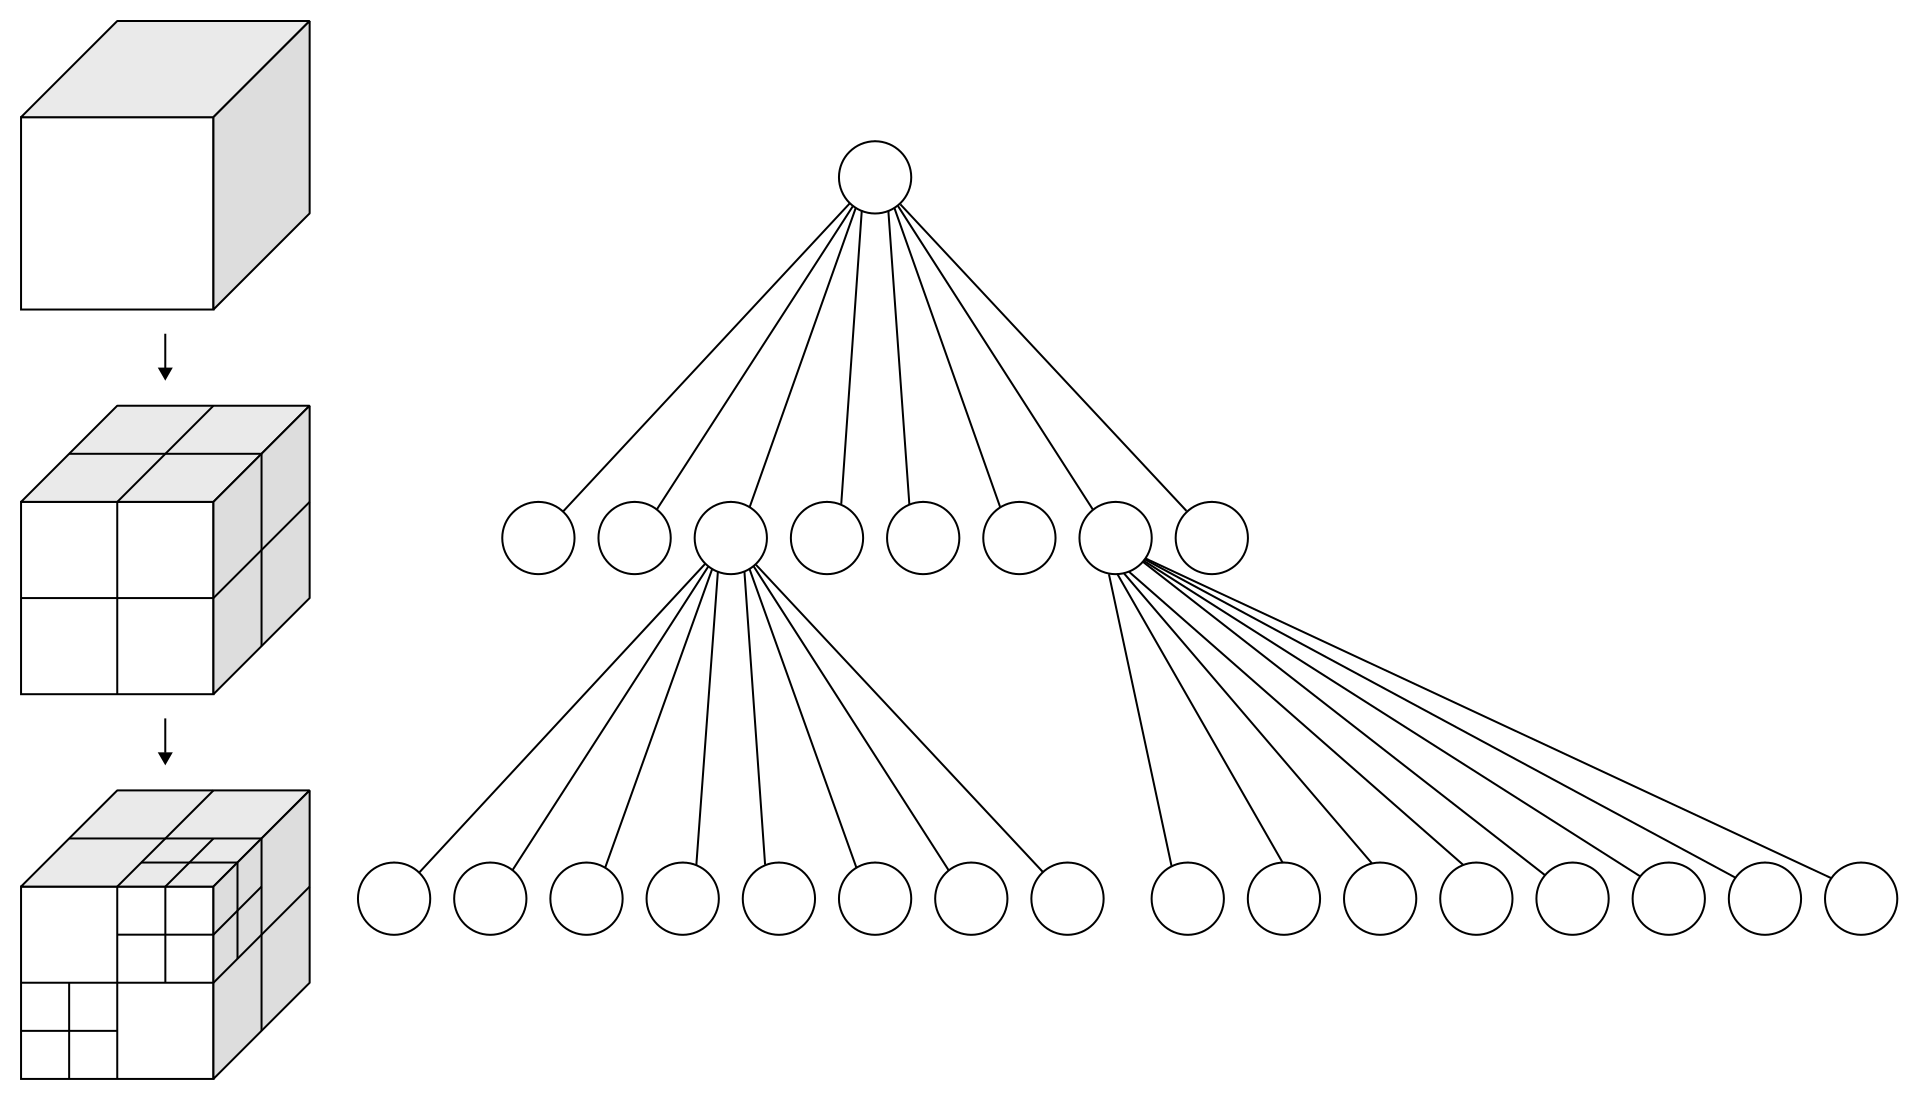
\includegraphics[scale=0.15]{octree.png}
	\end{center}
	\caption{Rekurzivno deljenje kocke na oktante.}
	\label{fig:oct}
\end{figure}



\subsection{Sweep and prune}
\label{subsec:sap}


\subsection{BSP}
\label{subsec:octree}


\section{Implementacija}
\label{sec:implementacija}


\section{Evaluacija}
\label{sec:evaluacija}

\section{Zaključak}
\label{sec:zakljucak}

Zaključak. 

\addcontentsline{toc}{section}{Literatura}
\appendix
\bibliography{bibl} 
\bibliographystyle{plain}

\appendix
\section{Dodatak}
Dodatak.
\end{document}
